\chapter{Experiment}
\label{chapter:experiment}

After StreamBench architecture and design of workloads are demonstrated, this chapter will draw our attention to experiments. Each experiment case is executed several times to get a stable result. In this chapter, we present experiment results of three selected stream processing systems running the workloads that are discussed in~\cref{section:workloads}. As illustrated in \cref{section:log_statistic}, two performance metrics that we are concerned with latency and throughput. For each workload, we compare the experiment results of different stream processing systems with visualization of these two metrics. 

\section{WordCount}
\label{section:wordcount_experiment}

First, we examine workload WordCount which aims to evaluate performance of stream processing systems performing basic operators. In order to check different performance metrics of stream processing systems, we performed the WordCount experiments in two different models: Offline model and Online model. Offline WordCount focuses on throughput and aims to find the corresponding maximum throughput of each systems. Offline means that the workload application consumes data that already exists in Kafka cluster. On the contrary, experiments consuming continuous coming data are Online model, which measures latency of stream processing with different throughputs. Moreover, we also made some modification to the original workload to evaluate pre-aggregation property of Storm.  As mentioned in~\cref{subsection:wordcount_generator}, for this workload, we designed two data generators to produce words that satisfy uniform and zipfian distributions. Comparison between experiment results of processing these two different data streams is also presented. 


\subsection{Offline WordCount}
\begin{figure}[t!]
  \begin{center}
  \subfigure[Skewed WordCount ]{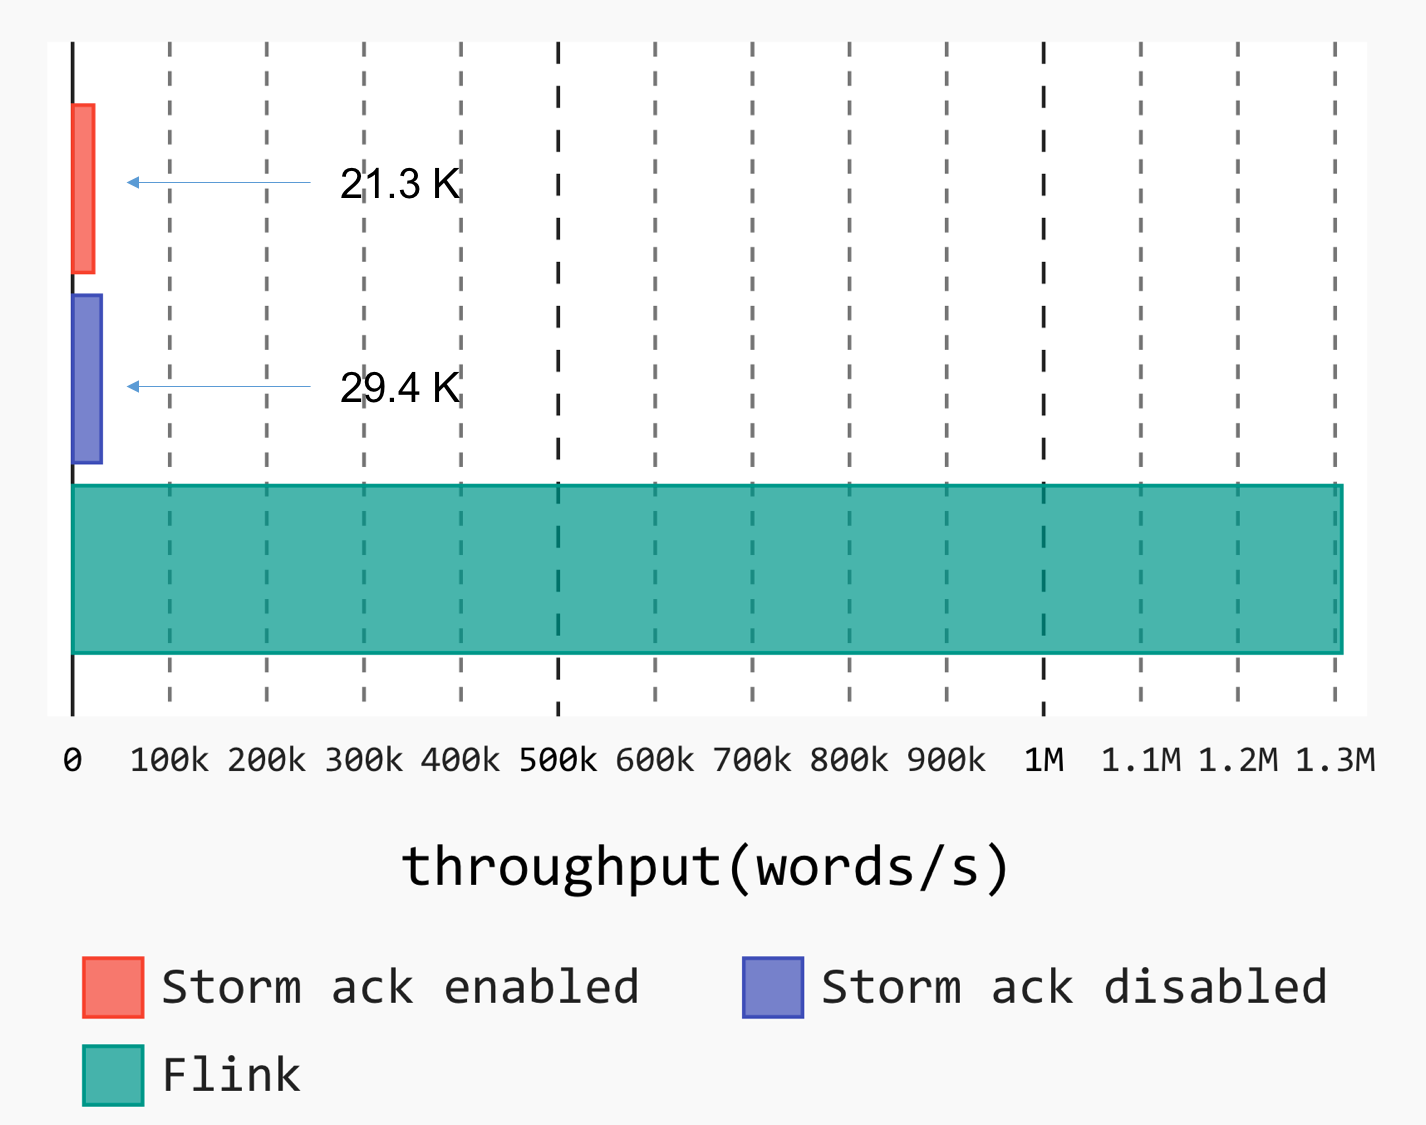
\includegraphics[scale=0.27]{images/throughput_skewed}}
  ~
  \subfigure[Uniform WordCount ]{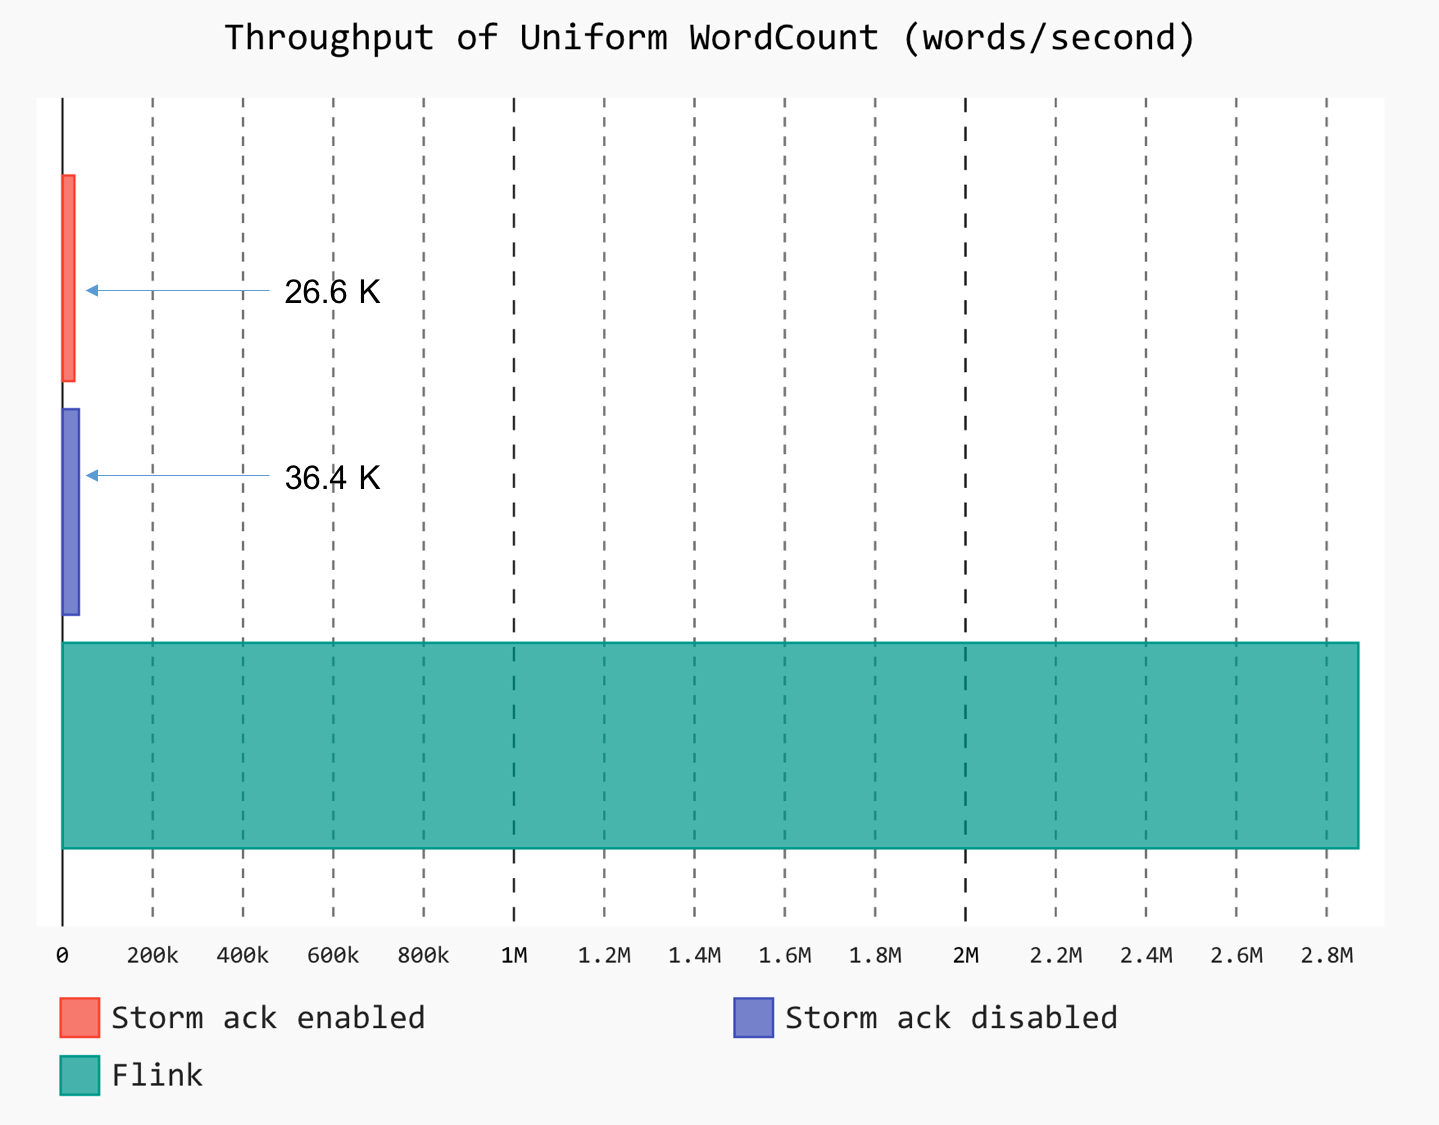
\includegraphics[scale=0.27]{images/throughput_uniform}}
   \caption{Throughput of Offline WordCount (words/second)}
   \label{fig:offline_throughput}
  \end{center}
\end{figure}

Since the computing model of Spark Streaming is micro-batch processing, existing data in Kafka cluster would be collected and processed as one single batch. The performance of processing one large batch with Spark Streaming is similar to a Spark batch job. There are already many works evaluating performance of Spark batch processing. Therefore, we skip experiments of Spark Streaming here. Figure~\ref{fig:offline_throughput} shows throughput of Storm and Flink clusters executing Offline WordCount with both skewed data and uniform data. It is obvious that the performance of Flink is much better than Storm, achieving around 50 to 100 times larger throughput. The throughput of Flink cluster processing uniform data stream up to 2.83 million words per second.  The skewness of experiment data has great influence of performance. The throughput of Flink cluster performing uniform data is more than two times as large as throughput of performing skewed data. The corresponding ratio of Storm is around 1.25. 

\begin{figure}[t!]
  \begin{center}
  \subfigure[Storm (ack enabled)]{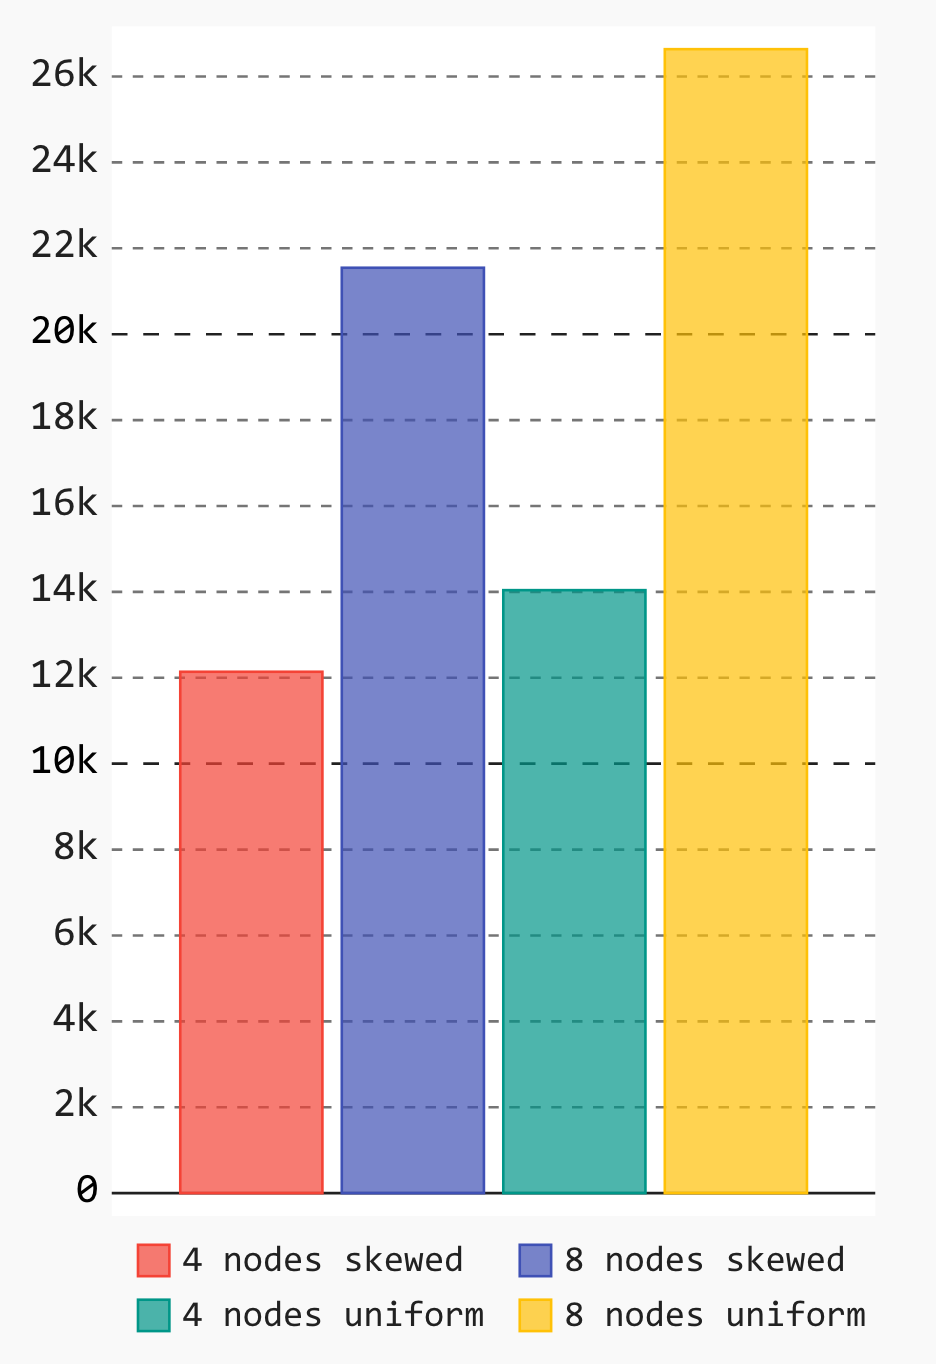
\includegraphics[scale=0.25]{images/storm_throughput_scale}}
  ~
  \subfigure[Flink]{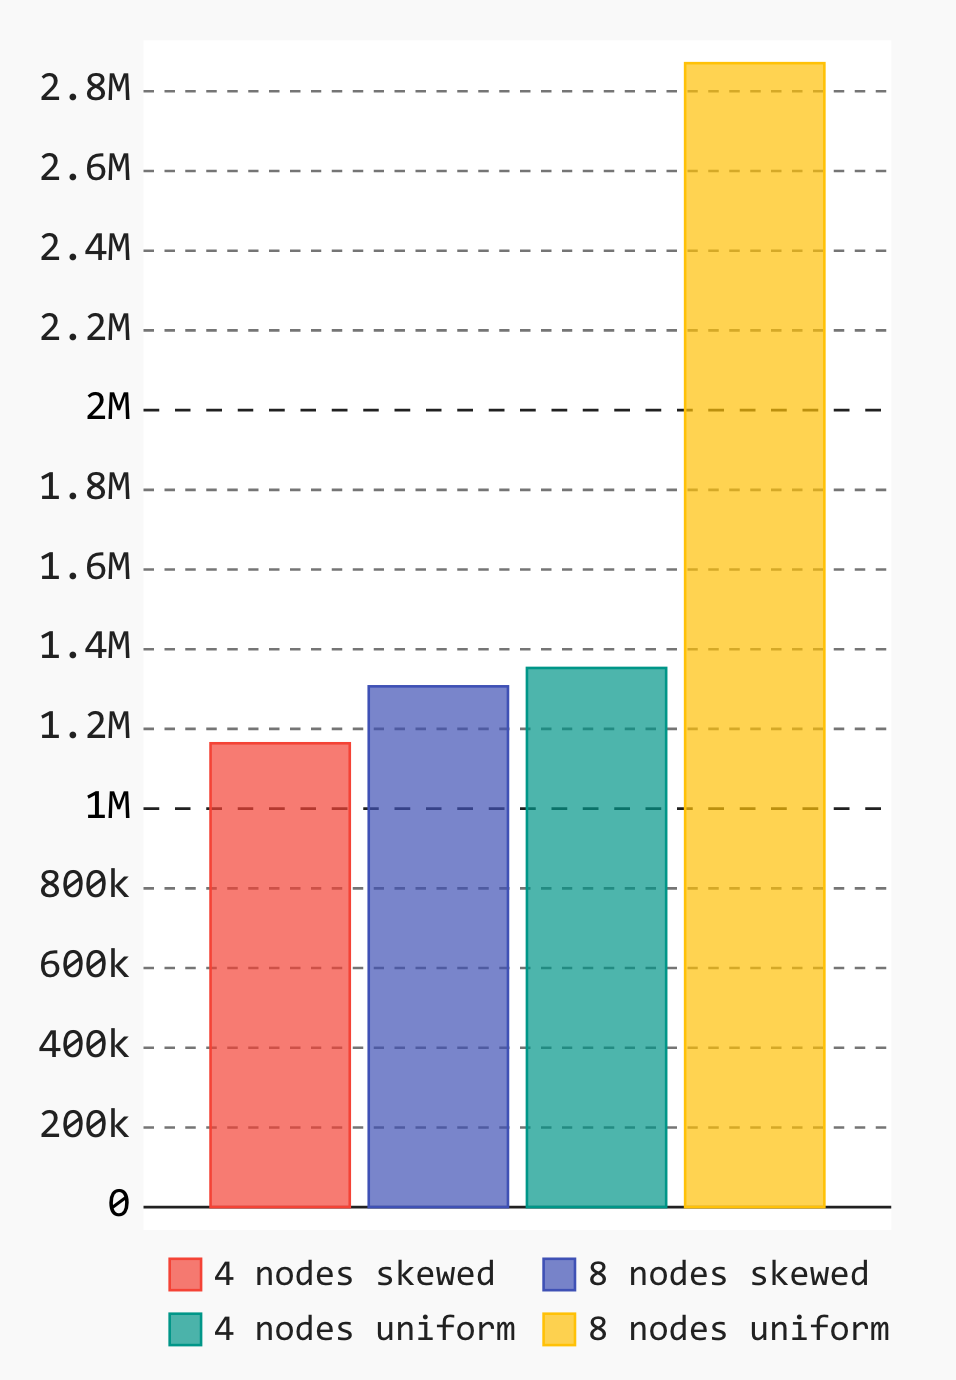
\includegraphics[scale=0.25]{images/flink_throughput_scale}}
   \caption{Throughput Scale Comparison of Offline WordCount}
   \label{fig:offline_throughput_scale}
  \end{center}
\end{figure}

The difference of performance between skewed data and uniform data indicates that the bottleneck of a cluster processing skewed data would be the node dealing with data with highest frequency. To verify this assumption, we reduce the number of computing nodes from 8 to 4, and run these experiments. The experiment results are presented as Figure~\ref{fig:offline_throughput_scale}. The throughput of 8-nodes cluster of both systems dealing with uniform data is nearly two times as large as that of 4-nodes cluster. It means that the scalability of both systems is good. While processing skewed data, increasing the number of work nodes in a Flink cluster doesn't bring significant performance increase. Storm cluster gets about 58\% throughput improvement while increasing cluster from 4 nodes to 8 nodes. These results show that the assumption is correct with Flink and the bottleneck of a storm cluster might be other factors.

The throughput of each work node in computing cluster is displayed in Figure~\ref{fig:worknodes_throughput}. Obviously storm has lower throughput, but achieves better workload balance than Flink. The experiment results also shows that clusters with 4 compute nodes of both systems have better workload balance than clusters with 8 nodes and workloads preforming uniform data achieve better balance that corresponding workloads performing skewed data.


\begin{figure}[t!]
  \begin{center}
   \subfigure{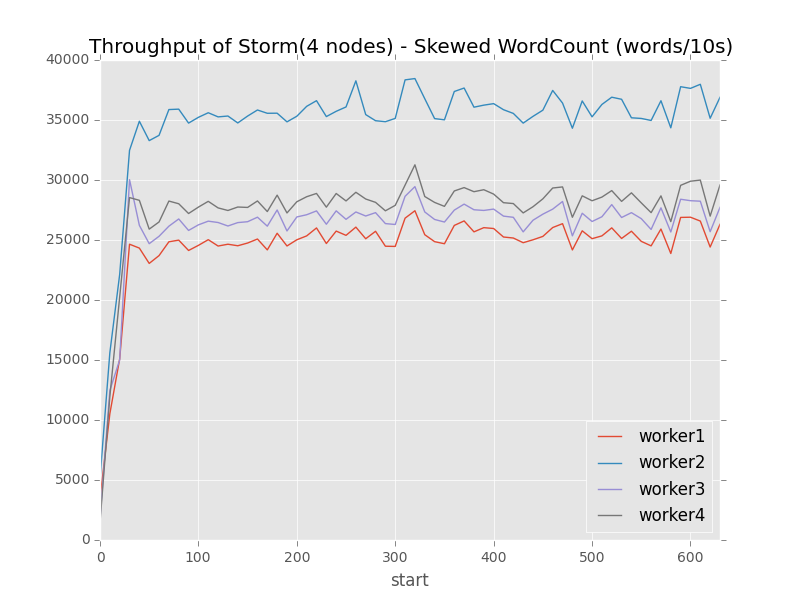
\includegraphics[scale=0.35]{images/storm4nodes_skewed_throughput}}
  ~
  \subfigure{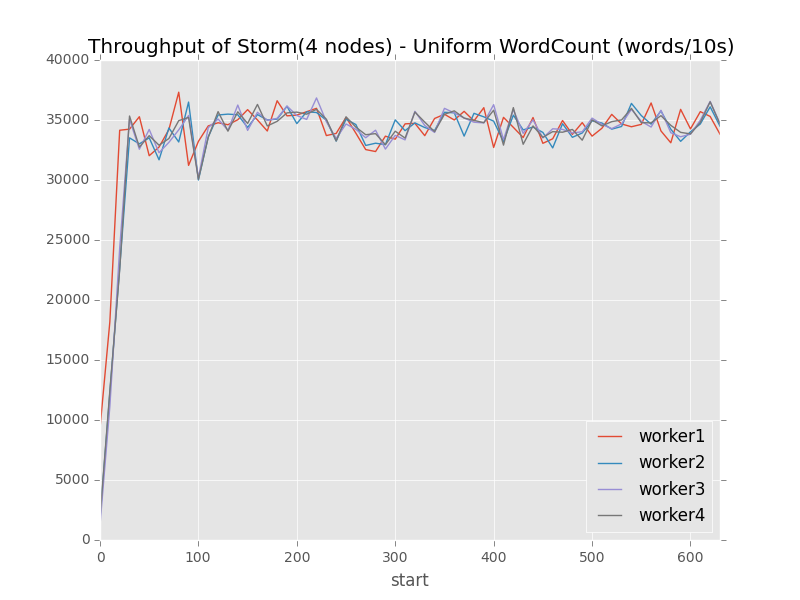
\includegraphics[scale=0.35]{images/storm4nodes_uniform_throughput}}
  ~
  \subfigure{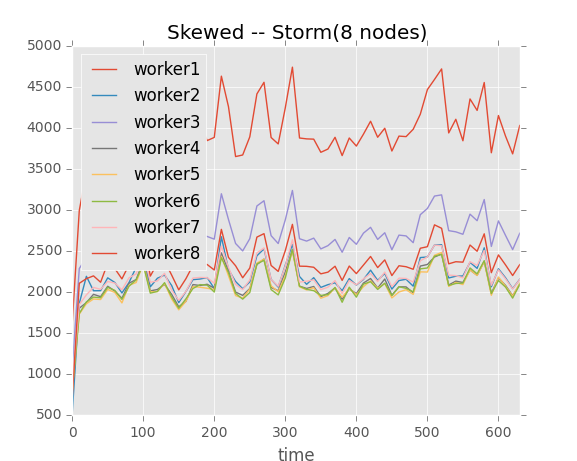
\includegraphics[scale=0.34]{images/storm_skewed_throughput2}}
  ~
  \subfigure{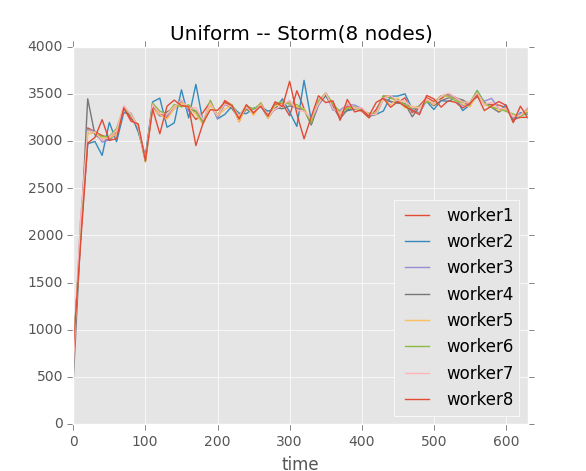
\includegraphics[scale=0.34]{images/storm_uniform_throughput2}}
  ~
    \subfigure{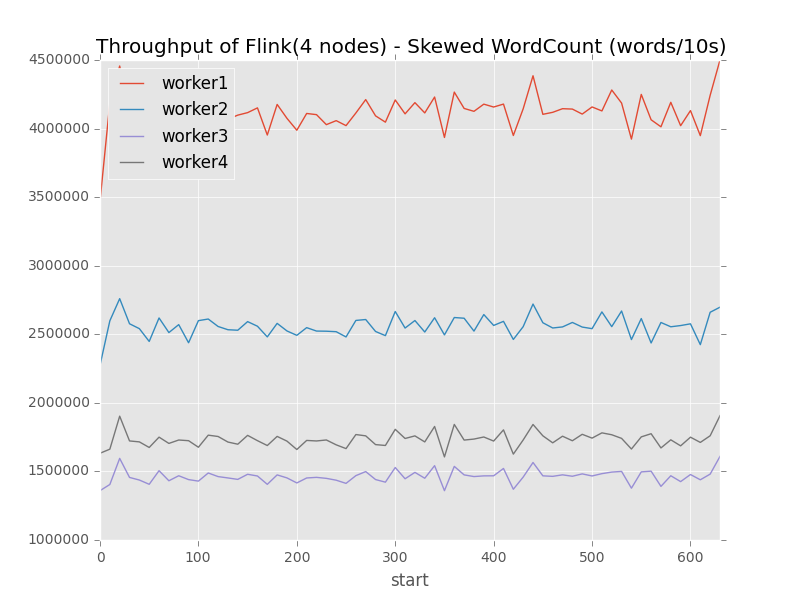
\includegraphics[scale=0.33]{images/flink4nodes_skewed_throughput}}
  ~
  \subfigure{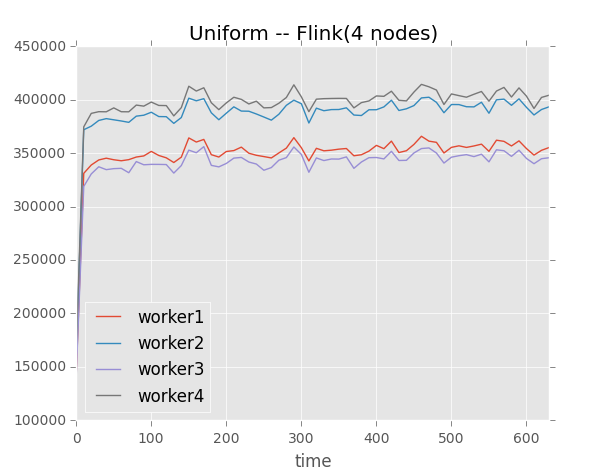
\includegraphics[scale=0.33]{images/flink4nodes_uniform_throughput}}
  ~
  \subfigure{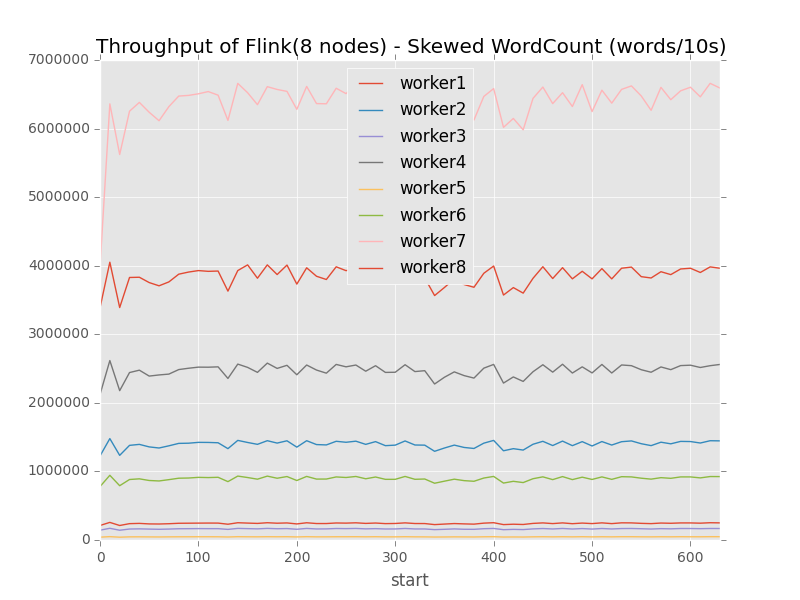
\includegraphics[scale=0.33]{images/flink_skewed_throughput}}
  ~
  \subfigure{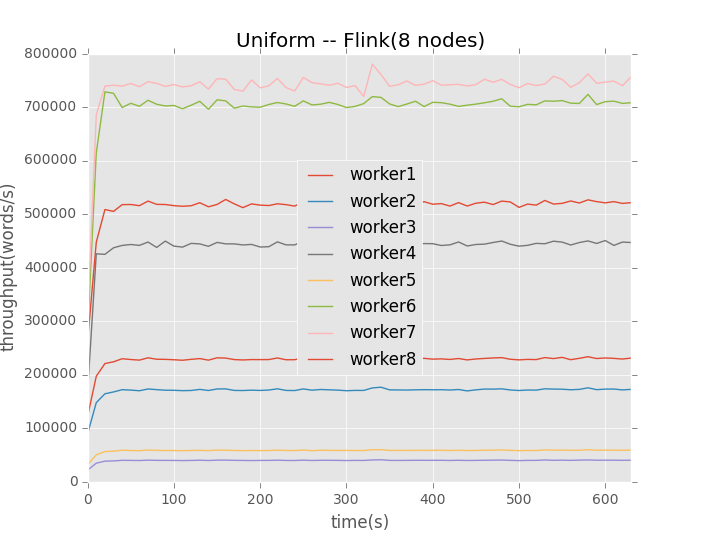
\includegraphics[scale=0.33]{images/flink_uniform_throughput}}

   \caption{Throughput of work nodes (words/s)}
   \label{fig:worknodes_throughput}
  \end{center}
\end{figure}

\subsection{Online WordCount}
\label{subsec:online_wordcount}

Base on the experiment results of Offline WordCount, we perform experiments of Online WordCount on Storm and Flink at around half of the maximum achieved throughput of Offline WordCount respectively. In Online scenario, the stream processing application starts earlier than data generation. Which means data is processed as soon as possible after it is generated. As mentioned in \cref{section:log_statistic}, the latency is computed as spending time from a record generated to corresponding result computed.

Figure~\ref{fig:online_wordcount_latency}\subref{fig:records} shows the latency of Online WordCount performing skewed data. Storm with ack enabled achieves a median latency of 10 milliseconds, and a 95-th percentile latency of 201 milliseconds, meaning that 95\% of all latencies were below 201 milliseconds. Flink has a higher median latency (39 milliseconds), and a similar 95-th percentile latency of 217 milliseconds. This Figure also presents the latency of Spark Streaming processing skewed words with half of the maximum throughput that is discussed below. Since the records  in a micro-batch are buffered up to batch interval time, the buffer time are also counted into the latency according to our latency computational method present in Figure~\ref{fig:latency}. Obviously, the latency of Spark Streaming is much higher than that of others.

% 99-th 521
\begin{figure}[t!]
  \begin{center}
  \subfigure[Records latency]{\label{fig:records}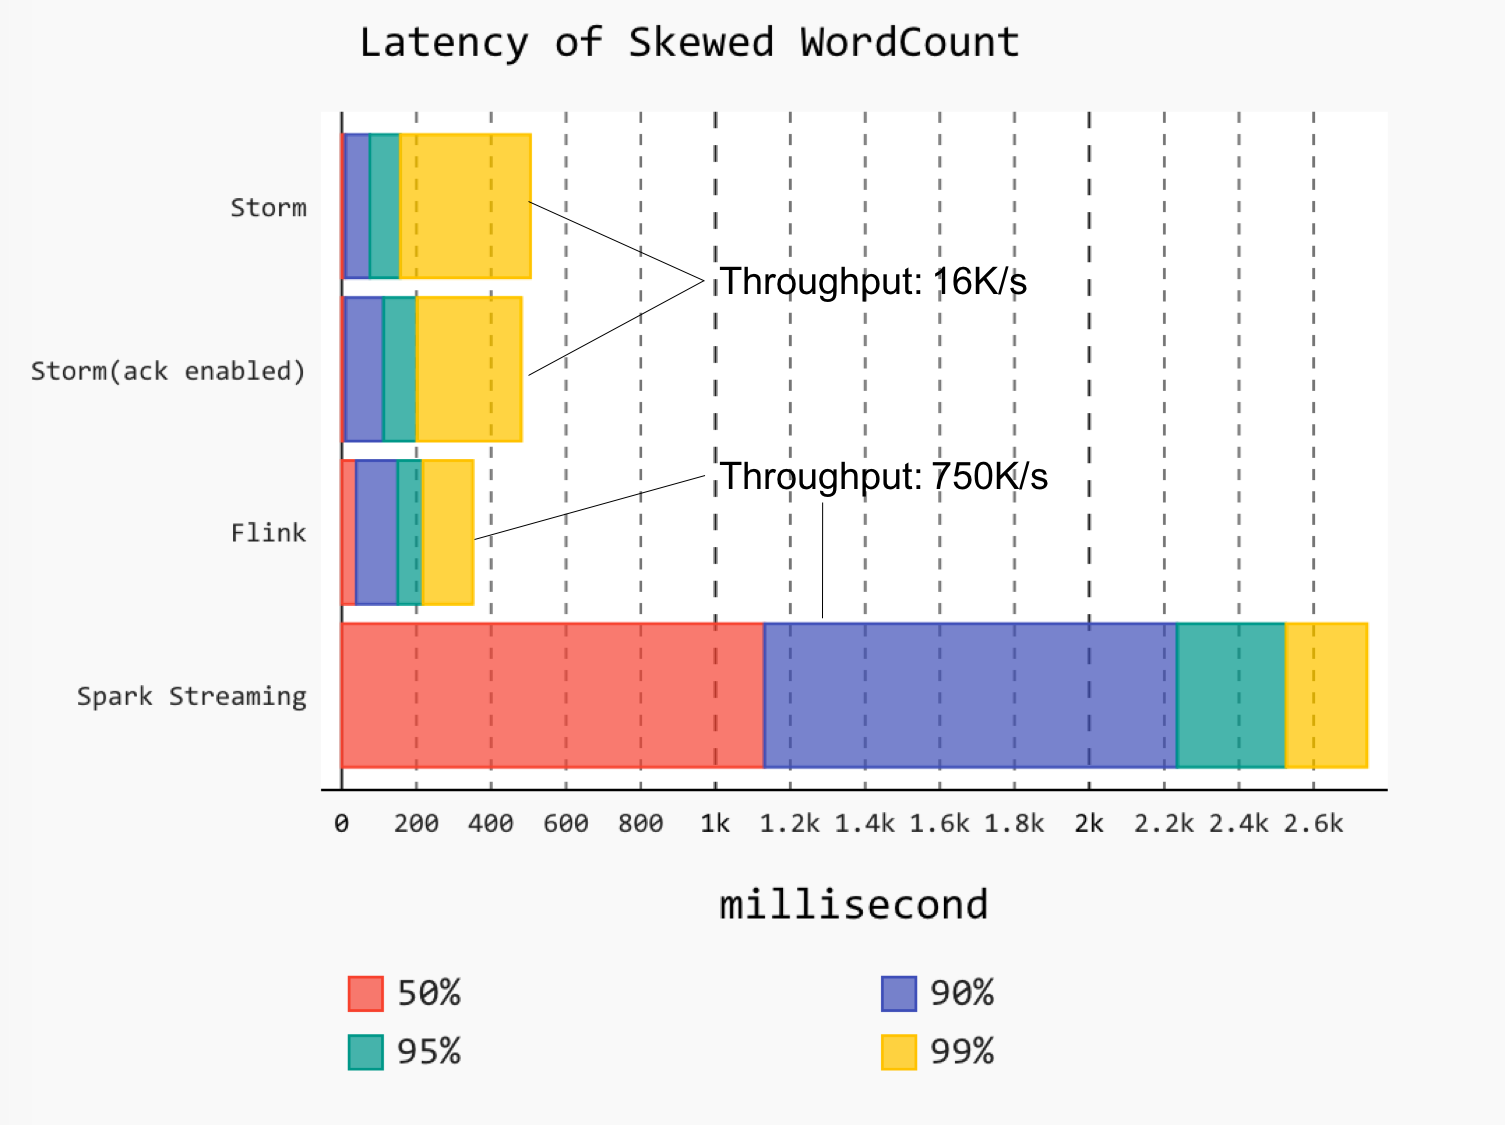
\includegraphics[scale=0.25]{images/latency_skewedwordcount}}
  \subfigure[Micro-batches latency]{\label{fig:batches}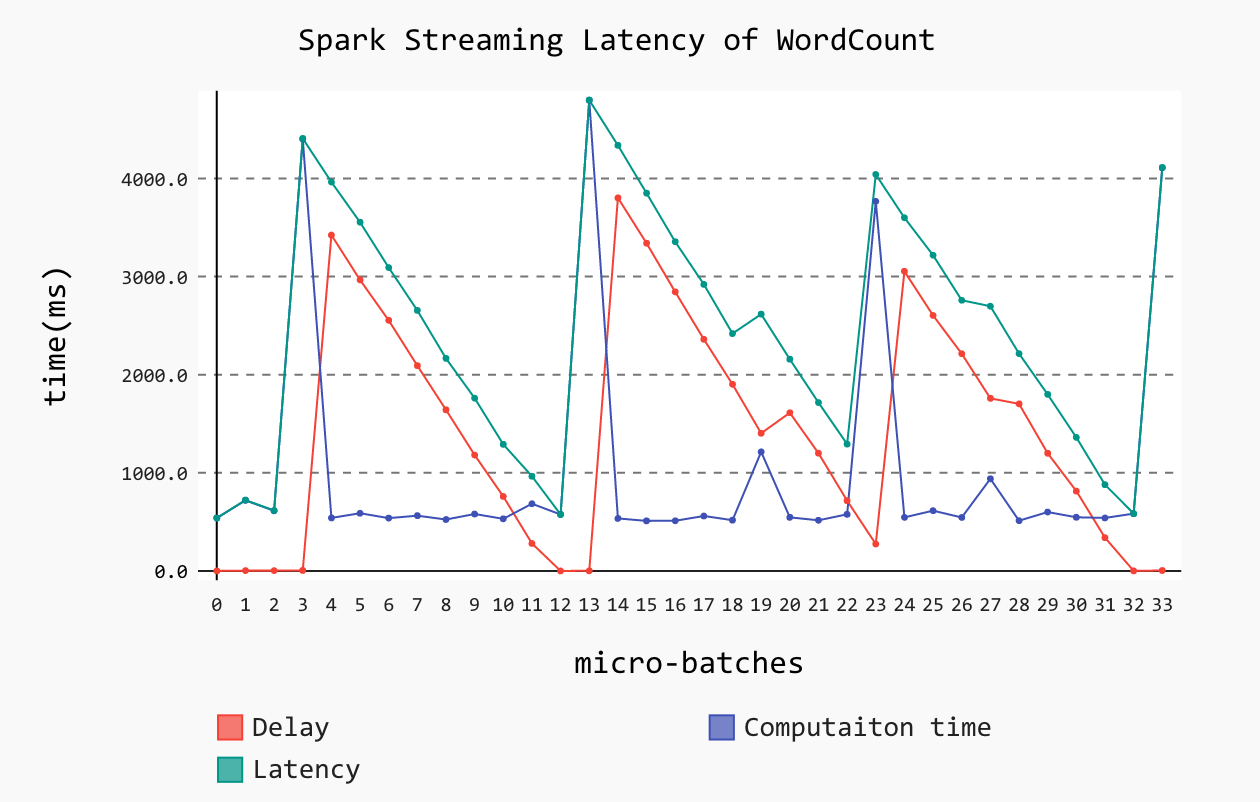
\includegraphics[scale=0.32]{images/spark_wordcount_latency}}
   \caption{Latency of Online WordCount}
   \label{fig:online_wordcount_latency}
  \end{center}
\end{figure}

In Spark Streaming, depending on the nature of the streaming computation, the batch interval used may have significant impact on the data rates that can be sustained by the application on a fixed set of cluster resources\footnote{\url{http://spark.apache.org/docs/1.5.1/streaming-programming-guide.html\#setting-the-right-batch-interval}}. Here, we perform the experiments with one second micro-batch interval and 10 seconds checkpoint interval which are the default configurations. Checkpointing is enabled because of a stateful transformation, \texttt{updateStateByKey} is used here to accumulate word counts.  Checkpointing is very time consuming due to writing information to a fault- tolerant storage system. Figure~\ref{fig:online_wordcount_latency}\subref{fig:batches} shows that the latency of micro-batches increasing and decreasing periodically because of checkpointing. In this Figure, window time of records in a micro-batch is not took in consideration. Before the computation of a micro-batch is finished, computation job of following micro-batches will not start. Therefore, the start time of computation job of a micro-batch would be delayed that is indicated by ``Delay" in the figure. The throughput of experiment corresponding to Figure~\ref{fig:online_wordcount_latency}\subref{fig:batches} is 1.4M/s (million words per second) of skewed data. When the speed of data generation reaches 1.8M/s, the delay and latency increase infinitely with periodic decreasing.

As mentioned in \cref{sub:basic_operator}, we designed another version of WordCount named Windowed Wordcount. Actually, Spark Streaming supports pre-aggregation by default, therefore, above Spark Streaming WordCount experiments already own this feature. Currently, Flink-0.10.1 doesn't support pre-aggregation, and parallel window can only be applied on keyed stream. It is possible to implement Windowed WordCount with Flink's low level API. But it is too time consuming and we leave it to future works. Therefore, only Storm is benchmarked with this workload.

%\begin{figure}
%  \begin{center}
%  \subfigure{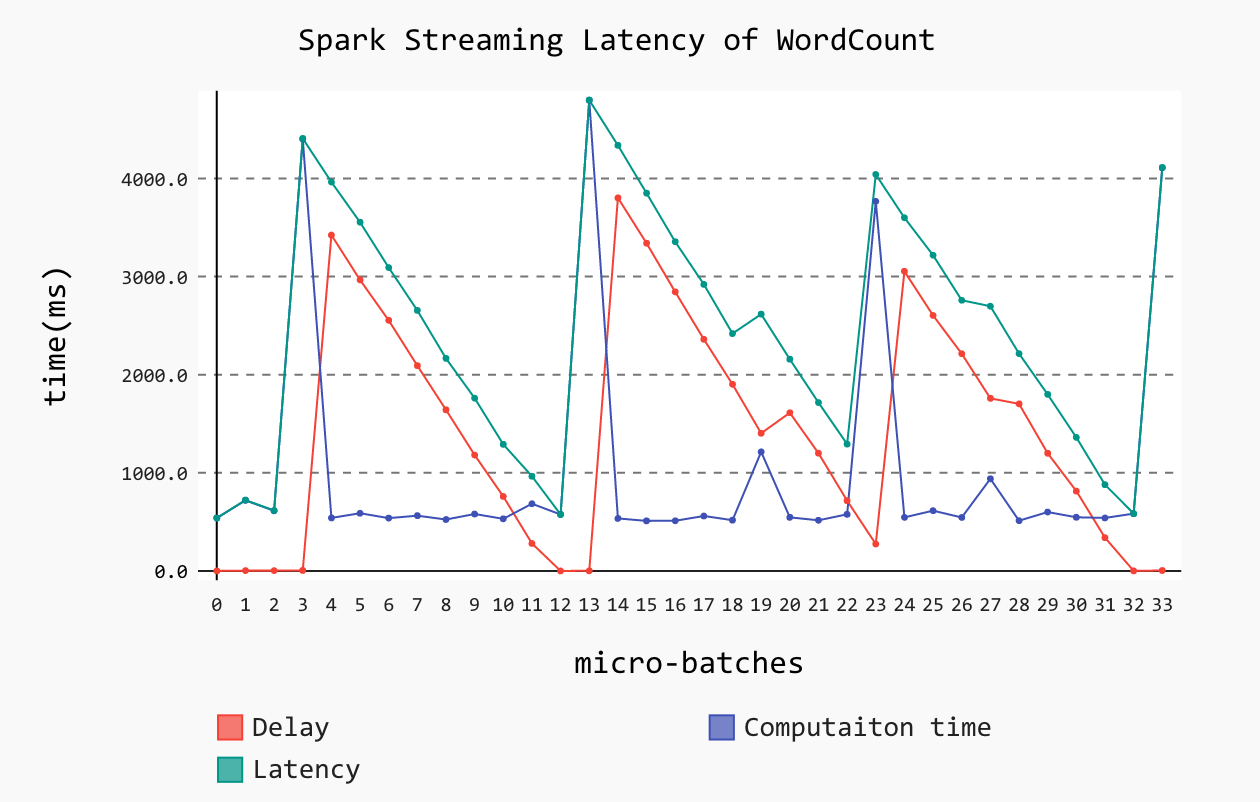
\includegraphics[scale=0.35]{images/spark_wordcount_latency}}
%   \caption{Spark Streaming WordCount Latency}
%   \label{fig:spark_wordcount_latency}
%  \end{center}
%\end{figure}

To support Windowed WordCount, we implemented a \texttt{window} operator in Storm\footnote{\url{https://github.com/wangyangjun/Storm-window}}. From our experiments, the window time has very limit effect on throughput. Here only experiment results of one second window workload are presented. The throughput of Windowed WordCount performing skewed data in Offline model could reach 60K/s (thousand words per second) that is more than two times as large as experiments without window. While dealing with uniform data, the throughput doesn't have any obvious improvement. Online model with a generation speed of 50K/s achieves a median latency of 1431 milliseconds, and a 99-th percentile latency of 3877 milliseconds.

Throughput of WordCount workload could be summarized as Table~\ref{table:wordcount_throughput}.

\begin{table}[H] %\centering
\begin{tabular}{P{2.6cm} | P{2.2cm} | P{2.2cm} | P{2.3cm} | P{2.3cm} } 
% Alignment of sells: l=left, c=center, r=right. 
% If you want wrapping lines, use p{width} exact cell widths.
% If you want vertical lines between columns, write | above between the letters
% Horizontal lines are generated with the \hline command:
\toprule % The line on top of the table
\hline
  & \multicolumn{2}{c|}{No Pre-aggregation}  & \multicolumn{2}{c}{Windowed Pre-aggregation} \\ 
\hline 
 & Uniform & Zipfian & Uniform & Zipfian \\
 \hline
% Place a & between the columns
% In the end of the line, use two backslashes \\ to break the line
% contents of the cell
 Storm  (ack disabled) &  36.4K & 29.4K & 50K & 60K \\ \hline
 Spark Streaming & $\O$ & $\O$ & 1.3M & 1.4M \\ \hline
 Flink & 2.8M & 1.4M & $\O$ & $\O$ \\ 
\hline
\bottomrule
\end{tabular} % for really simple tables, you can just use tabular
% You can place the caption either below (like here) or above the table
\caption{WordCount Throughput} 
% Place the label just after the caption to make the link work
\label{table:wordcount_throughput}
\end{table}


\section{AdvClick}

\begin{figure}
  \begin{center}
  \subfigure{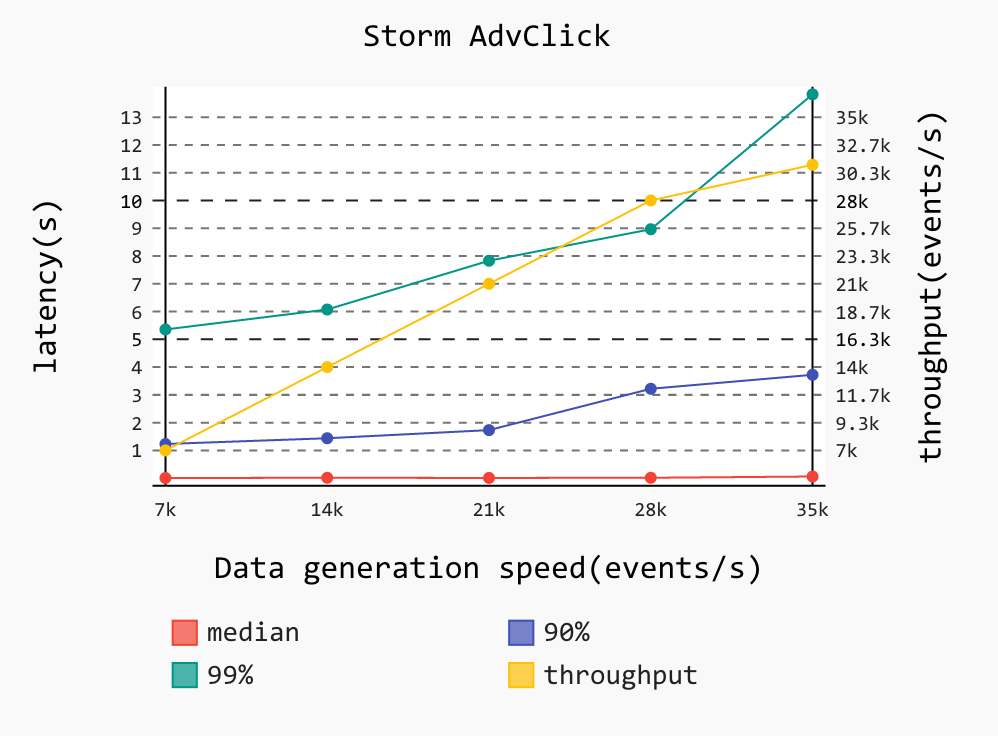
\includegraphics[scale=0.45]{images/storm_adv_latency}}
   \caption{Storm AdvClick Performance}
   \label{fig:storm_adv_click}
  \end{center}
\end{figure}

As described in \cref{subsection:advclick_generator}, click delays of clicked advertisements satisfy normal distribution and the mean is set to 10 seconds. In our experiments, we define that clicks in 20s after corresponding advertisement shown are valid clicks. In theory, overwhelming majority records in stream \texttt{click} could be joined. Kafka only provides a total order over messages within a partition, not between different partitions in a topic \cite{Kafka}. Therefore, it is possible that click record arrives earlier than corresponding advertisement shown record. We set a window time of 5 seconds for \texttt{advertisement clicks} stream.

When benchmarking Storm and Flink, first we perform experiments with low speed data generation and then increase the speed until obvious joining failures occur when throughput is much less than generation speed of stream \texttt{advertisement clicks}. The experiment result shows that the maximum throughput of Storm cluster is around 8.4K/s (joined events per second). The corresponding generation speed of \texttt{shown advertisements} is 28K/s. As we can see in Figure~\ref{fig:storm_adv_click}, cluster throughput of  \texttt{shown advertisements} is equal to the data generation speed  when it is less than 28K/s. Figure~\ref{fig:storm_adv_click} also shows that Storm cluster has a very low median latency. The 90-th percentiles of latency are all between one second and two seconds. But the 99-th percentile of latency are much higher and increase dramatically with the data generation speed.

\begin{figure}
  \begin{center}
  \subfigure{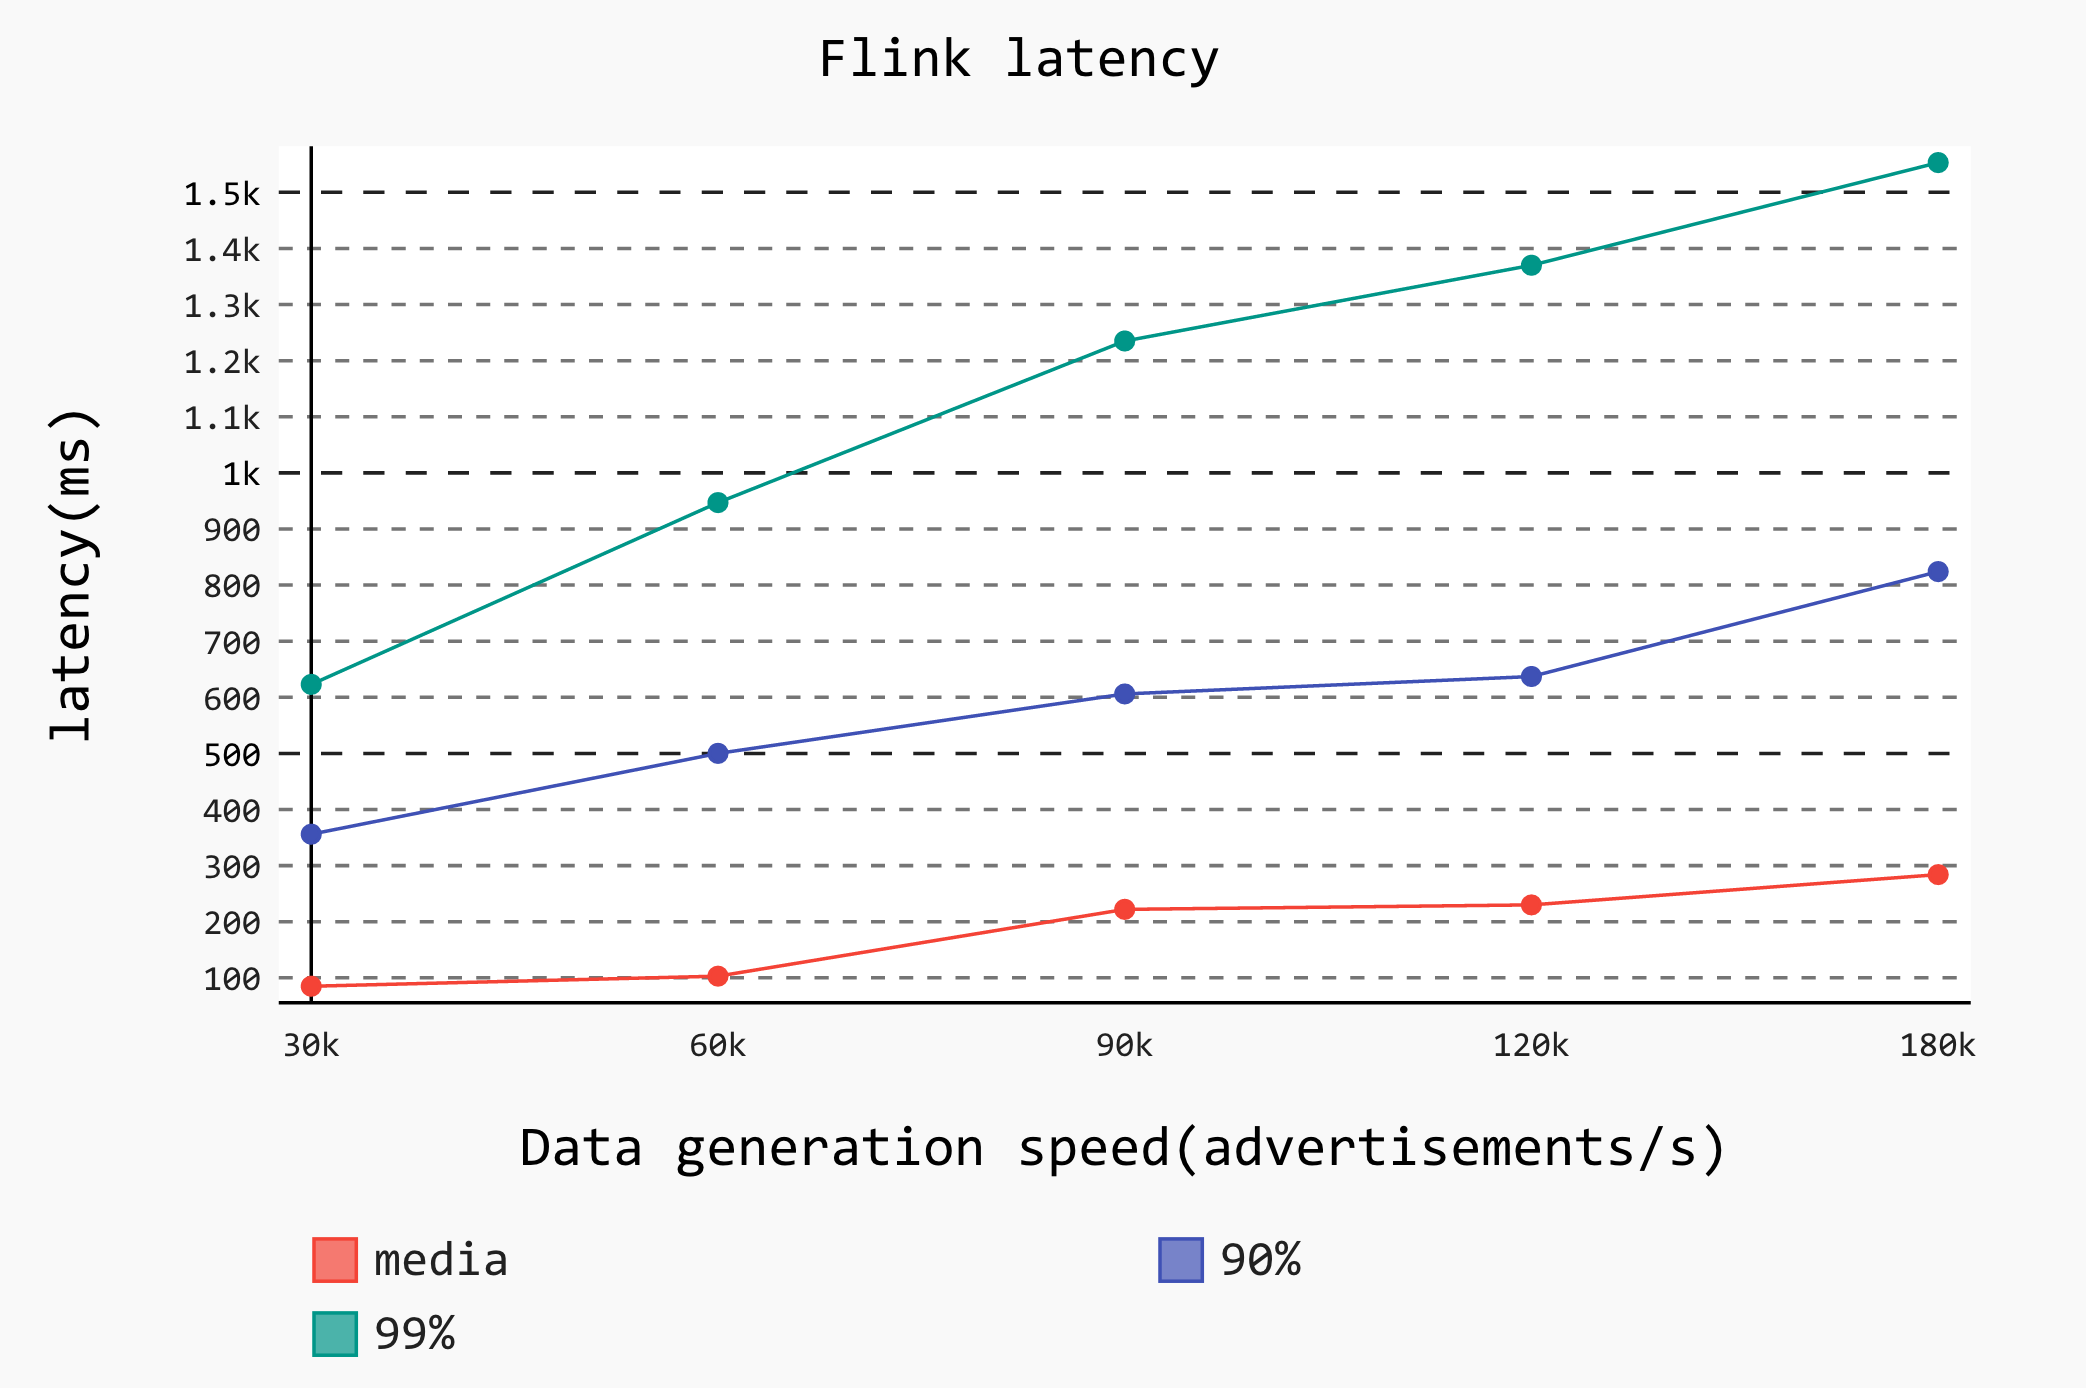
\includegraphics[scale=0.25]{images/flink_adv_latency}}
   \caption{Flink AdvClick Latency}
   \label{fig:flink_adv_click}
  \end{center}
\end{figure}


%Compared to Storm, Flink achieves a much better throughput. When generation speed of stream \texttt{shown advertisements} increases from 180K/s to 210K/s, Flink cluster stops consuming data from Kafka. The maximum throughput of Flink is between 54 K/s and 63K/s, around 6 times larger than Storm. The latency of Flink performing this workload is shown as Figure~\ref{fig:flink_adv_click}. Even though the median latencies are a little higher than Storm, but 90-th and 99-th percentiles of Flink latency are much lower. 

Compared to Storm, Flink achieves a much better throughput. In our experiments, the throughput of Flink cluster is always equal to the generation speed of stream \texttt{shown advertisements}. But when the generation speed of stream \texttt{shown advertisements} is larger than 200K/s, the Flink AdvClick processing job is usually failed because of a bug in flink-connector-kafka \footnote{\url{https://issues.apache.org/jira/browse/KAFKA-725}}. This issue is fixed in the latest versions of Flink and Kafka. But Storm and Spark don't support the latest version Kafka yet. We will upgrade all these systems in StreamBench in the future. The maximum throughput of Flink we achieved in experiments is 63K/s (joined events per second), around 6 times larger than Storm. The latency of Flink performing this workload is shown as Figure~\ref{fig:flink_adv_click}. Even though the median latencies are a little higher than Storm, but 90-th and 99-th percentiles of Flink latency are much lower. 

As discussed in \cref{sub:join_operator}, Spark Streaming join operator is applied with sliding window. With the configuration of 20s/5s, the slide intervals of both windows are 5 seconds. That means a micro-batch join job is submitted to Spark Streaming cluster every 5 seconds. Because of different processing model, there is no joining failure in Spark Streaming. But high data generation speed leads to increasing delay of micro-batch jobs because the previous micro-batch jobs couldn't be finished in interval time. With this configuration, Spark Streaming has a very small throughput which is lower than 2K/s. Increasing micro-batch jobs submitting interval might increase the throughput, but leads to higher latency. For this workload, increasing the window lengths also gives up correctness of results. Therefore, we did some experiments with larger windows. Increasing windows length of these two streams to 60s/30s, the cluster could achieve a throughput of 20K/s which is ten times larger. 

\begin{table}[H] %\centering
\begin{tabular}{P{4cm} | P{2.3cm} | P{2.3cm} | P{3cm} } 
\toprule % The line on top of the table
\hline
  System & Throughput  & Median Latency & 90-th Percentile Latency \\ 
\hline 
% Place a & between the columns
% In the end of the line, use two backslashes \\ to break the line
% contents of the cell
 Storm (ack disabled) &  8.4K/s & 10ms & 1438ms \\ \hline
 Flink & 63K/s & 230ms & 637ms \\ \hline
 Spark Streaming (20s/5s) & \textless~2K/s & $\O$ &  $\O$  \\ \hline
 Spark Streaming (60s/30s) & 20K/s & $\sim$~15s+20s &  $\sim$~27s+24s  \\

\hline
\bottomrule
\end{tabular} % for really simple tables, you can just use tabular
% You can place the caption either below (like here) or above the table
\caption{Advertisement Click Performance} 
% Place the label just after the caption to make the link work
\label{table:AdvClick}
\end{table}

Table~\ref{table:AdvClick} summarizes maximum throughputs and latencies at half of corresponding maximum throughput achieved by these systems. Flink achieves the largest throughput and lowest 90-th percentile latency. While the median latency of Storm is a median latency of 10ms, that is much lower than other systems.

\section{K-Means}

Experiment results of stream k-means processing 2-dimensional points shows that Storm cluster with at-least-once processing guarantee has a throughput of 1.7K/s. Without this guarantee, the throughput is a litter larger, around 2.7K/s. The maximum throughput of Flink cluster is much larger and reaches 78K/s. Figure~\ref{fig:kmeans_latency} shows the latencies of Flink cluster and Storm Cluster without at-least-once guarantee. When the generation speed of point stream is low, Storm achieves very low median latency. The 90-th percentile of latency of Storm is also a little lower than Flink. The latency of Storm rises sharply when the generation speed is around 2.7K/s to 3K/s. Compare with Storm, latency percentiles of Flink is more compact. When the speed of data generations is 30K/s, Flink achieves a median latency of 141 milliseconds, and a 90-th percentile latency of 195 milliseconds. From this figure, it is easy to know that the throughput of Flink is significantly larger than storm.

%Figure~\ref{fig:kmeans_latency} shows the latencies of Storm and Flink clusters operating at around half size of corresponding max throughput. Both Storm with and without at-least-once guarantee achieve very low median latency and a much higher 99-th percentile latency. Generally, the latency of Storm with at-lest-once guarantee is a little higher. Compare with Storm, latency percentiles of Flink is more compact. Flink achieves a median latency of 122 milliseconds, and a 99-th percentile latency of 310 milliseconds. 
 
\begin{figure}
  \begin{center}
  \subfigure{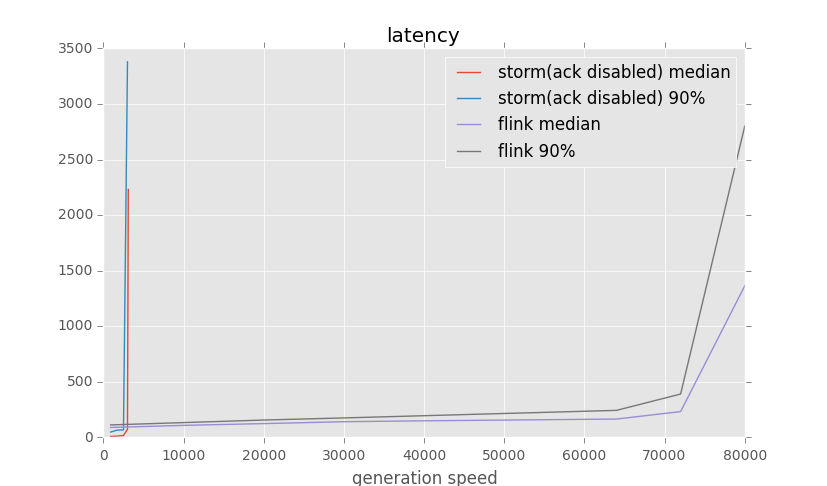
\includegraphics[scale=0.4]{images/kmeans_flink_storm_latency}}
   \caption{KMeans Latency of Flink and Storm}
   \label{fig:kmeans_latency}
  \end{center}
\end{figure}

% convance
Since the throughput of Flink is tens of times higher than Storm, this workload converges much quicker on Flink cluster. In order to compare convergences of the algorithm running on Storm and Flink clusters, we calculated average distance between centroids and corresponding nearest center over the number of points processed on each compute node and visualized as Figure~\ref{fig:converge} \subref{fig:flink_storm}. The results indicate that the k-means algorithm performing on Storm cluster achieves significantly better convergence.


% dimension
Our experiment results show that increasing point dimension has very limit effect on workload performance. The main effect of high point dimension is increasing computation in point distance calculation. Which indicates that computation is not a bottleneck of this workload. 
%Compared with low point dimension, high dimension leads to larger record size and more computation in point distance calculation. Which indicates that computation is not a bottleneck of this workload. 

\begin{figure}[t!]
  \begin{center}
   \subfigure[Flink and Storm]{\label{fig:flink_storm}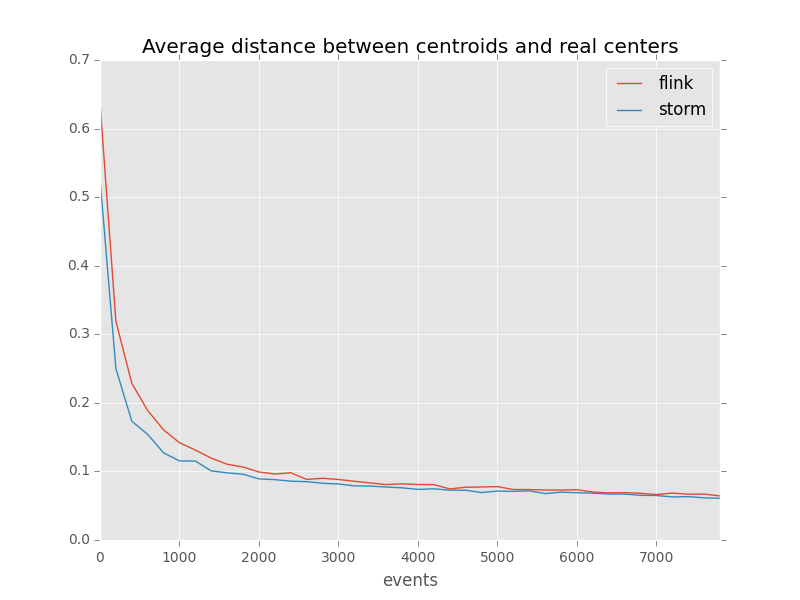
\includegraphics[scale=0.4]{images/converge}}
  ~
  \subfigure[Spark Streaming]{\label{fig:spark}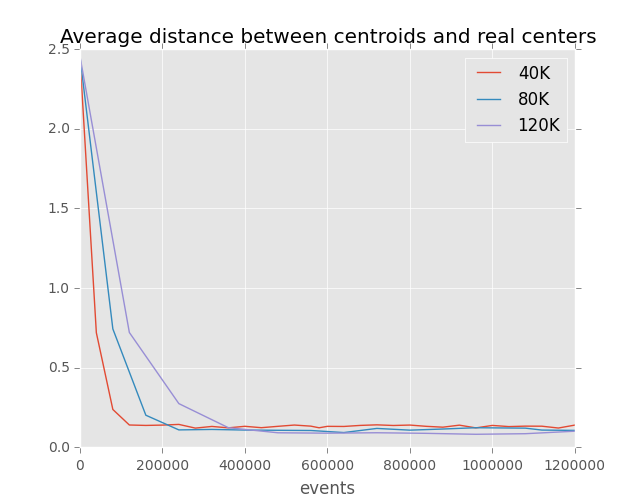
\includegraphics[scale=0.4]{images/converge_spark}}
   \caption{Convergences}
   \label{fig:converge}
  \end{center}
\end{figure}

Because of Spark's DAG computational model, Spark Streaming doesn't support iterate operator. Instead of forwarding updated centroids in a nested cycle, Spark Streaming implements stream k-means in a different way. It maintains a clustering model and updates the model with each micro batch processed. The update interval of clustering model is the same as micro batch interval. More detail about Spark Streaming K-Means could be found online\footnote{\url{https://databricks.com/blog/2015/01/28/introducing-streaming-k-means-in-spark-1-2.html}}. With the default setting of one second micro-batch interval, the maximum throughput of the cluster could reach 1M/s so that the average latency of micro-batches is less than one second. The average latencies of micro-batches processing data with different generation speed are shown as Figure~\ref{fig:spark_kmeans_latency}. The latency of a micro-batch is the time from when the batch is ready to the time that the processing job is done. The latency of each record also includes the time that the record buffered in a window.
The experiment results show that the convergence of Spark Streaming K-Means is very fast. Usually, it is converged in a few micro-batches. Figure~\ref{fig:converge} \subref{fig:spark} shows the convergence of Spark Streaming over processed events,processing point streams with different generation speed. It is obvious that stream with lower speed converges faster. But stream with higher speed achieves lower average distance between centroids and real centers after converged.
 
%spark latency
\begin{figure}
  \begin{center}
  \subfigure{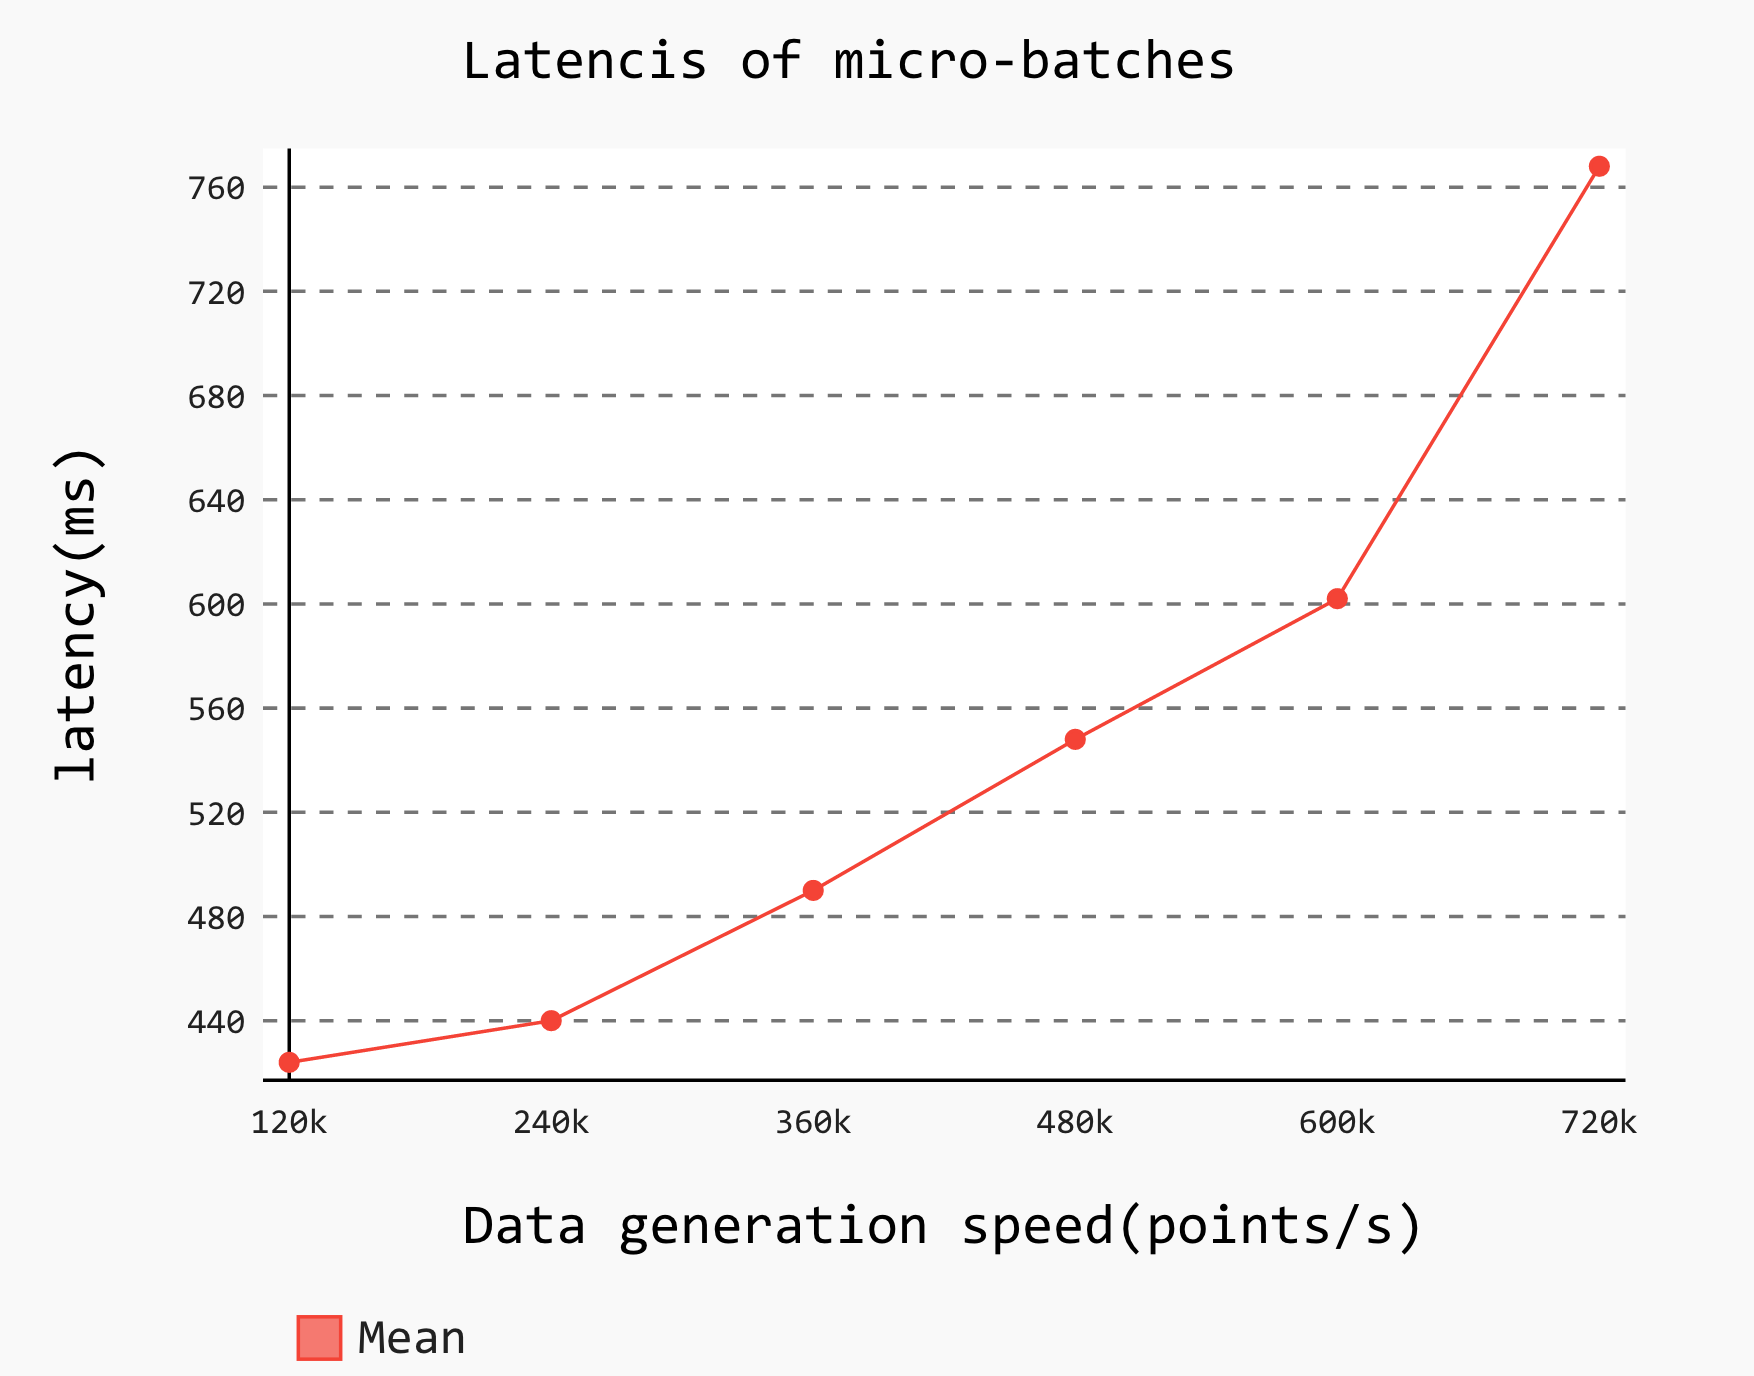
\includegraphics[scale=0.24]{images/spark_kmeans_latency}}
   \caption{Spark KMeans Latency}
   \label{fig:spark_kmeans_latency}
  \end{center}
\end{figure}

\begin{table}[H] %\centering
\begin{tabular}{P{2.2cm} | P{2.2cm} | P{2cm} | P{1.5cm} | P{1.5cm} | P{1.5cm}} 
\toprule % The line on top of the table
\hline 
  System & Maximum  &  \multicolumn{3}{c}{Latency} \\  \cline{3-6}
  & Throughput & Throughout & Median & 90\% & 99\% \\ \hline 
 Storm (ack enabled) &  1.7K/s & 0.9K/s & 13ms & 100ms & 410ms \\ \hline
 Storm (ack disabled) &  2.7K/s & 1.6K/s & 21ms & 107ms & 388ms \\ \hline 
 Flink & 78K/s & 40K/s & 122ms & 183ms & 310ms \\ \hline
 Spark Streaming & 1M/s & 480K/s & 986ms & 1271ms & 1837ms \\

\hline
\bottomrule
\end{tabular} % for really simple tables, you can just use tabular
% You can place the caption either below (like here) or above the table
\caption{KMeans Performance} 
% Place the label just after the caption to make the link work
\label{table:kmenas}
\end{table}

The performance of this workload is summarized in Table~\ref{table:kmenas}. It is clear that Spark Streaming achieves the best maximum throughput, and Storm achieves the lowest median latency.
\section{Summary}

The experiment results shows that both Flink and Spark Streaming achieve much higher throughput than Storm. But Storm achieves a very low median latency. Generally, median latency of Flink is a litter higher than Storm. But they 99-th percentile latency are similar and usually less than one second. The computational model of Spark Streaming is micro-batch, that leads to a tradeoff between throughput and latency. The latency of Spark Streaming is usually much larger than Storm and Flink. 

In practice, the selection of stream processing systems depends on the situation. If an application requests very low latency, but the requirement of throughput is not stringent, Storm would be the best choice. On the contrary, if throughput is the key requirement, Spark Streaming is a very good option. Flink achieves both low latency and high throughput. For most stream processing cases, Flink would be a good choice. 

\clearpage



